\documentclass{article}
\usepackage{amsmath}
\usepackage{amssymb}
\usepackage{graphicx}
\usepackage{hyperref}
\usepackage[version=4]{mhchem}


\begin{document}
\section*{Problem}
Both \(\triangle A B C\) and \(\triangle A D C\) are right triangles sharing the hypotenuse \(A C\) with \(\angle A B C=\angle A D C=90^{\circ}\). Points \(M\) and \(n\) are the midpoints on sides \(A C\) and \(B D\), respectively. Show that \(M N \perp B D\).\\
\centering
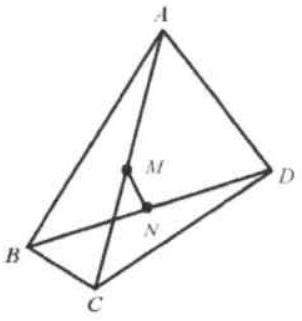
\includegraphics[width=\textwidth]{images/016(3).jpg}

\section*{Solution}
(D).\\
\(\triangle A B D\) is 3:4:5 right triangle. Since \(B D=25, A D=15\), and \(A B=20\).\\
We know that\\
\(C D^{2}=B D \times D E \Rightarrow \quad 20^{2}=25 \times D E \Rightarrow \quad D E=16\)

Draw \(A F \perp B D\). \(\frac{A F \times B D}{2}=\frac{A D \times A B}{2}\)\\
\centering
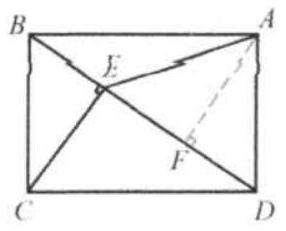
\includegraphics[width=\textwidth]{images/095.jpg}

\[
\Rightarrow \frac{A F \times 25}{2}=\frac{15 \times 20}{2} \Rightarrow A F=12
\]

The area of \(\triangle A D E\) is \(\frac{A F \times E D}{2}=\frac{12 \times 20}{2}=120\).\\

\end{document}
